% https://tex.stackexchange.com/a/403723
\documentclass[xcolor={dvipsnames,svgnames,table}, 8pt]{beamer}
\usepackage{tikz}
\begin{document}
\begin{frame}
    \frametitle{Test}
    \begin{columns}
    \begin{column}{.3\textwidth}
    \centering
    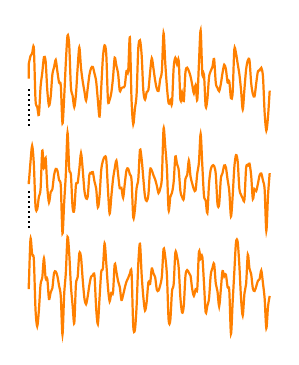
\begin{tikzpicture}[
    declare function={
      excitation(\t,\w) = sin(\t*\w);
      noise = rnd - 0.5;
      source(\t) = excitation(\t,20) + noise;
      filter(\t) = 1 - abs(sin(mod(\t, 50)));
      speech(\t) = 1 + source(\t)*filter(\t);
    }
  ]
    \draw[orange, thick, x=0.0085cm, y=.5cm] (0,1) -- plot [domain=0:360, samples=144, smooth] (\x,{speech(\x)});
    \draw[densely dotted, thick] (0,1.2) -- (0,1.7);
    \draw[orange, thick, x=0.0085cm, y=.5cm,yshift=1.3cm] (0,1) -- plot [domain=0:360, samples=144, smooth] (\x,{speech(\x)});
    \draw[densely dotted, thick] (0,2.5) -- (0,3.0);
    \draw[orange, thick, x=0.0085cm, y=.5cm,yshift=2.6cm] (0,1) -- plot [domain=0:360, samples=144, smooth] (\x,{speech(\x)});
     \end{tikzpicture}
    \end{column}
    \end{columns}
\end{frame}
\end{document}
